\documentclass[tikz,border=5mm]{standalone}
\usetikzlibrary{decorations.pathreplacing}

\begin{document}
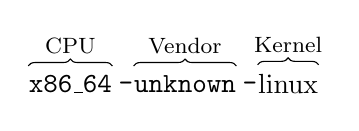
\begin{tikzpicture}
    {
        % Draw the target triplet
        \node[inner xsep=0pt,align=left] (cpu) {\texttt{x86\textunderscore64}};
        \node[inner xsep=0pt,anchor=west,right=2pt] at (cpu.east) (dash1) {\texttt{-}};
        \node[inner xsep=0pt,anchor=west] at (dash1.east) (vendor) {\texttt{unknown}};
        \node[inner xsep=0pt,anchor=west,right=2pt] at (vendor.east) (dash2) {\texttt{-}};
        \node[inner xsep=0pt,anchor=west] at (dash2.east) (os) {\textnormal{linux}};
    }

    % Draw the annotations with brackets
    \draw[decorate,decoration={brace,mirror}] (cpu.north east) -- node[above=1pt] {\footnotesize\textnormal{CPU}} (cpu.north west);
    \draw[decorate,decoration={brace,mirror}] (vendor.north east) -- node[above=1pt] {\footnotesize\textnormal{Vendor}} (vendor.north west);
    \draw[decorate,decoration={brace,mirror}] (os.north east) -- node[above=1pt] {\footnotesize\textnormal{Kernel}} (os.north west);
\end{tikzpicture}
\end{document}